% ── Esquemas de Ciencias (TikZ) ───────────────────────────────────────────────
% Diagramas propios para las láminas de solución. Cada uno dibuja solo lo que dice
% el temario DEMRE 2027 (scripts/pipeline/temario/ciencias.py). Monocromos con un
% acento: se leen igual impresos en blanco y negro.
\usetikzlibrary{arrows.meta,calc,positioning}
\tikzset{esq/.style={font=\scriptsize\sffamily, line width=0.6pt, >={Stealth[length=4pt]}},
  caja/.style={draw=zinc700, rounded corners=2pt, inner sep=3pt, align=center, font=\scriptsize\sffamily},
  cajaac/.style={caja, draw=acento, line width=1pt}}
\newcommand{\resistencia}[2]{\draw[fill=white, draw=acento, line width=0.9pt] ($(#1)+(-0.28,-0.1)$) rectangle ($(#1)+(0.28,0.1)$); \node[font=\tiny, above=1pt] at (#1) {#2};}
\newcommand{\resistenciav}[2]{\draw[fill=white, draw=acento, line width=0.9pt] ($(#1)+(-0.1,-0.28)$) rectangle ($(#1)+(0.1,0.28)$); \node[font=\tiny, right=3pt] at (#1) {#2};}
\newcommand{\pila}[1]{\draw[line width=1pt] ($(#1)+(-0.06,-0.14)$) -- ($(#1)+(-0.06,0.14)$); \draw[line width=1pt] ($(#1)+(0.06,-0.24)$) -- ($(#1)+(0.06,0.24)$);}

\newcommand{\esqSerie}{\begin{tikzpicture}[esq]
  \draw (0,0) rectangle (3,1.6); \fill[white] (-0.1,0.6) rectangle (0.1,1.0); \pila{0,0.8}
  \resistencia{1,1.6}{$R_1$} \resistencia{2,1.6}{$R_2$}
  \node[align=center, anchor=north] at (1.5,-0.12) {serie: la misma corriente\\los voltajes se suman\\$R = R_1 + R_2$};
\end{tikzpicture}}

\newcommand{\esqParalelo}{\begin{tikzpicture}[esq]
  \draw (0,0) rectangle (3,1.6); \draw (1.5,0) -- (1.5,1.6); \fill[white] (-0.1,0.6) rectangle (0.1,1.0); \pila{0,0.8}
  \resistenciav{1.5,0.8}{$R_1$} \resistenciav{3,0.8}{$R_2$}
  \node[align=center, anchor=north] at (1.5,-0.12) {paralelo: el mismo voltaje\\las corrientes se suman\\$R$ eq.\ menor que cada una};
\end{tikzpicture}}

\newcommand{\esqOnda}{\begin{tikzpicture}[esq]
  \draw[zinc500] (0,0) -- (4.2,0);
  \draw[acento, line width=1pt, domain=0:4, samples=80] plot (\x,{0.55*cos(\x*180)});
  \draw[<->] (0,0.85) -- node[above] {$\lambda$} (2,0.85);
  \draw[dashed, zinc500] (2,0) -- (2,0.55); \node[right] at (2,0.28) {$A$};
  \node[align=center, anchor=north] at (2.1,-0.7) {$c = \lambda\, f$ \quad $T = 1/f$\\más frecuencia, menor $\lambda$};
\end{tikzpicture}}

\newcommand{\esqReflexion}{\begin{tikzpicture}[esq]
  \draw[line width=1.2pt] (0,0) -- (3.4,0); \node[below] at (3.0,0) {espejo};
  \draw[dashed, zinc500] (1.7,0) -- (1.7,1.8); \node[above] at (1.7,1.8) {normal};
  \draw[->, acento, line width=1pt] (0.5,1.5) -- (1.7,0); \draw[->, line width=1pt] (1.7,0) -- (2.9,1.5);
  \node at (1.4,0.9) {$\theta_i$}; \node at (2.0,0.9) {$\theta_r$};
  \node at (1.7,-0.7) {$\theta_i = \theta_r$ (desde la normal)};
\end{tikzpicture}}

\newcommand{\esqRefraccion}{\begin{tikzpicture}[esq]
  \fill[zinc200] (0,-1.5) rectangle (3.4,0); \draw (0,0) -- (3.4,0);
  \node[right] at (0,0.25) {medio 1}; \node[right] at (0,-0.3) {medio 2 (más lento)};
  \draw[dashed, zinc500] (1.7,1.5) -- (1.7,-1.5);
  \draw[->, acento, line width=1pt] (0.6,1.4) -- (1.7,0); \draw[->, acento, line width=1pt] (1.7,0) -- (2.25,-1.4);
  \node at (1.45,0.75) {$\theta_1$}; \node at (1.9,-0.8) {$\theta_2$};
  \node[align=center] at (1.7,-2.0) {se acerca a la normal;\\la frecuencia no cambia};
\end{tikzpicture}}

\newcommand{\esqCicloCelular}{\begin{tikzpicture}[esq]
  \draw[line width=2pt] (90:1) arc (90:-40:1); \draw[line width=2pt] (-44:1) arc (-44:-140:1);
  \draw[line width=2pt] (-144:1) arc (-144:-210:1); \draw[acento, line width=3pt] (-214:1) arc (-214:-266:1);
  \node at (25:1.35) {$G_1$}; \node at (-92:1.3) {$S$}; \node at (-177:1.35) {$G_2$}; \node[acento] at (122:1.3) {$M$};
  \node[align=center] at (0,0) {interfase\\[-1pt]\tiny en $S$ se\\[-2pt]\tiny replica el ADN};
  \node[align=left, anchor=west] at (1.75,0.3) {mitosis: $2n \rightarrow$ 2 células $2n$\\[1pt]meiosis: $2n \rightarrow$ 4 células $n$};
\end{tikzpicture}}

\newcommand{\esqFotosintesis}{\begin{tikzpicture}[esq]
  \node[cajaac, minimum width=1.9cm, minimum height=0.8cm] (c) at (0,0) {cloroplasto\\fotosíntesis};
  \node[caja, minimum width=1.9cm, minimum height=0.8cm] (m) at (3.6,0) {mitocondria\\respiración};
  \draw[->] ($(c.east)+(0,0.18)$) -- node[above] {glucosa + O$_2$} ($(m.west)+(0,0.18)$);
  \draw[->] ($(m.west)+(0,-0.18)$) -- node[below] {CO$_2$ + H$_2$O} ($(c.east)+(0,-0.18)$);
  \draw[->, acento] (0,1.1) -- node[right] {luz} (c.north); \draw[->] (m.south) -- node[right] {ATP} (3.6,-1.1);
\end{tikzpicture}}

\newcommand{\esqTectonica}{\begin{tikzpicture}[esq]
  \draw[line width=1pt] (0,1) -- (2,1) -- (3.6,-0.4); \draw (0,0.7) -- (1.9,0.7) -- (3.3,-0.6);
  \draw[line width=1pt] (2,1) -- (2.6,1.15) -- (3,1.6) -- (3.3,1.3) -- (4.4,1.1);
  \node[font=\tiny, align=center] at (0.8,1.25) {placa de Nazca}; \node[font=\tiny, align=center] at (3.9,0.75) {placa\\Sudamericana};
  \draw[->, acento] (0.3,1.5) -- (1.3,1.5);
  \fill[acento] (2.6,0.45) circle (2pt); \node[right, font=\tiny] at (2.65,0.35) {hipocentro};
  \draw[dashed] (2.6,0.45) -- (2.6,1.15); \fill (2.6,1.15) circle (1.6pt); \node[above left, font=\tiny] at (2.6,1.15) {epicentro};
  \node at (2.2,-0.95) {borde convergente: subducción};
\end{tikzpicture}}

\newcommand{\esqDivergente}{\begin{tikzpicture}[esq]
  \draw[line width=1pt] (0,0.8) -- (1.8,0.8); \draw[line width=1pt] (2.4,0.8) -- (4.2,0.8);
  \draw (0,0.4) -- (1.8,0.4); \draw (2.4,0.4) -- (4.2,0.4);
  \draw[->, acento, line width=1pt] (1.6,1.15) -- (0.6,1.15); \draw[->, acento, line width=1pt] (2.6,1.15) -- (3.6,1.15);
  \fill[acento!25] (1.85,0.85) -- (2.35,0.85) -- (2.2,-0.6) -- (2.0,-0.6) -- cycle; \node[font=\tiny] at (2.1,-0.8) {magma};
  \node[align=center] at (2.1,-1.35) {dorsal: las placas se separan\\y se forma nuevo suelo oceánico};
\end{tikzpicture}}

\newcommand{\esqKepler}{\begin{tikzpicture}[esq]
  \draw (0,0) ellipse (1.9 and 1.05); \fill[acento] (-1.15,0) circle (3.5pt); \node[below] at (-1.15,-0.1) {Sol};
  \fill (-1.9,0) circle (1.5pt); \node[left] at (-1.9,0) {perihelio}; \fill (1.9,0) circle (1.5pt); \node[right] at (1.9,0) {afelio};
  \node[align=center] at (0,-1.5) {más rápido cerca del Sol\\áreas iguales en tiempos iguales};
\end{tikzpicture}}

\newcommand{\esqMovimiento}{\begin{tikzpicture}[esq]
  \draw[->] (0,0) -- (1.9,0) node[below] {$t$}; \draw[->] (0,0) -- (0,1.5) node[left] {$x$};
  \draw[acento, line width=1pt] (0,0.2) -- (1.7,1.3); \node[align=center] at (0.95,-0.5) {MRU\\pendiente = velocidad};
  \begin{scope}[xshift=2.6cm]
  \fill[acento!20] (0,0) -- (1.7,0) -- (1.7,1.3) -- cycle;
  \draw[->] (0,0) -- (1.9,0) node[below] {$t$}; \draw[->] (0,0) -- (0,1.5) node[left] {$v$};
  \draw[acento, line width=1pt] (0,0) -- (1.7,1.3); \node[align=center] at (0.95,-0.5) {MRUA\\área = desplazamiento};
  \end{scope}
\end{tikzpicture}}

\newcommand{\esqFuerzas}{\begin{tikzpicture}[esq]
  \draw (-1.6,0) -- (1.6,0); \draw[line width=0.9pt] (-0.5,0) rectangle (0.5,0.6);
  \draw[->, line width=1pt] (0,0.3) -- (0,-0.9) node[below] {$P = mg$};
  \draw[->, line width=1pt] (0,0.6) -- (0,1.5) node[above] {$N$};
  \draw[->, acento, line width=1pt] (0.5,0.35) -- (1.5,0.35) node[right] {$F$};
  \draw[->, line width=1pt] (-0.5,0.12) -- (-1.3,0.12) node[left] {$f_r=\mu N$};
  \node[align=left, anchor=west] at (2.3,0.3) {$F_{\text{neta}} = m\,a$\\$F_{\text{neta}}=0$: reposo o $v$ constante};
\end{tikzpicture}}

\newcommand{\esqAtomo}{\begin{tikzpicture}[esq]
  \draw[zinc500] (0,0) circle (0.6); \draw[zinc500] (0,0) circle (1.05); \draw[acento, line width=1pt] (0,0) circle (0.22);
  \node[font=\tiny] at (0,0) {p$^+$n$^0$};
  \foreach \a in {0,180} \fill (\a:0.6) circle (1.6pt); \foreach \a in {90,210,330} \fill (\a:1.05) circle (1.6pt);
  \node[align=left, anchor=west] at (1.35,0.1) {$Z$ = protones\\$A$ = protones + neutrones\\neutrones $= A - Z$\\isótopos: igual $Z$, distinto $A$\\catión: perdió e$^-$ · anión: ganó e$^-$};
\end{tikzpicture}}

\newcommand{\esqCarbono}{\begin{tikzpicture}[esq]
  \foreach \y/\n/\h/\g in {1/1/sp^3/tetraédrica, 0.5/2/sp^2/plana, 0/3/sp/lineal} {
    \node at (0,\y) {C}; \node at (1.2,\y) {C};
    \ifnum\n=1 \draw (0.15,\y) -- (1.05,\y); \fi
    \ifnum\n=2 \draw (0.15,\y+0.04) -- (1.05,\y+0.04); \draw[acento] (0.15,\y-0.04) -- (1.05,\y-0.04); \fi
    \ifnum\n=3 \draw (0.15,\y) -- (1.05,\y); \draw[acento] (0.15,\y+0.06) -- (1.05,\y+0.06); \draw[acento] (0.15,\y-0.06) -- (1.05,\y-0.06); \fi
    \node[anchor=west] at (1.5,\y) {$\h$ \quad \g}; }
  \node at (1.6,-0.55) {cada doble enlace aporta un enlace $\pi$};
\end{tikzpicture}}

\newcommand{\esqMol}{\begin{tikzpicture}[esq]
  \node[caja] (g) at (0,0) {masa (g)}; \node[cajaac] (n) at (2,0) {moles ($n$)}; \node[caja] (p) at (4.1,0) {partículas ($N$)};
  \draw[->] (g) -- node[below=2pt] {$\div M$} (n); \draw[->] (n) -- node[below=2pt] {$\times 6{,}02\cdot10^{23}$} (p);
  \node at (2,-0.85) {los coeficientes de la ecuación relacionan moles};
\end{tikzpicture}}

\newcommand{\esqDilucion}{\begin{tikzpicture}[esq]
  \foreach \x/\h/\t in {0/0.5/{C_1,\,V_1}, 2.4/0.95/{C_2,\,V_2}} {
    \fill[acento!18] (\x+0.05,0.05) rectangle (\x+0.95,\h); \draw (\x,1.3) -- (\x,0) -- (\x+1,0) -- (\x+1,1.3); \node at (\x+0.5,-0.25) {$\t$}; }
  \draw[->, acento] (1.15,0.65) -- node[above, font=\tiny] {+ disolvente} (2.25,0.65);
  \node[align=center, anchor=north] at (1.7,-0.5) {$C_1V_1 = C_2V_2$\\los moles de soluto no cambian};
\end{tikzpicture}}

\newcommand{\esqNeurona}{\begin{tikzpicture}[esq]
  \foreach \x in {0,3.3} {
    \foreach \a in {140,170,200,230} \draw ($(\x,0)+(\a:0.2)$) -- ++(\a:0.4); \draw (\x,0) circle (0.2); }
  \draw[acento, line width=1.2pt] (0.2,0) -- (2.6,0); \foreach \a in {-30,0,30} \draw (2.6,0) -- ++(\a:0.25);
  \node[below, font=\tiny] at (-0.4,-0.35) {dendritas}; \node[above] at (1.4,0.05) {axón};
  \draw[<->, zinc500] (2.88,-0.35) -- (3.0,-0.35); \node[below, font=\tiny, align=center] at (2.95,-0.38) {sinapsis:\\neurotransmisores};
  \node[font=\tiny] at (1.6,0.75) {dos neuronas: células separadas};
\end{tikzpicture}}

\newcommand{\esqReflejo}{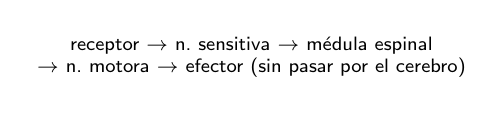
\begin{tikzpicture}[esq]
  \node[align=center] at (0,0) {receptor $\rightarrow$ n.\ sensitiva $\rightarrow$ médula espinal\\$\rightarrow$ n.\ motora $\rightarrow$ efector (sin pasar por el cerebro)};
\end{tikzpicture}}

\newcommand{\esqInvestigacion}{\begin{tikzpicture}[esq, node distance=0.25cm]
  \node[caja] (a) {observación}; \node[caja, right=of a] (b) {pregunta}; \node[caja, right=of b] (c) {hipótesis};
  \node[caja, below=0.5cm of a] (d) {diseño:\\variables y control}; \node[caja, right=of d] (e) {resultados}; \node[cajaac, right=of e] (f) {conclusión};
  \draw[->] (a) -- (b); \draw[->] (b) -- (c); \draw[->] (c.south) -- ++(0,-0.15) -| (d.north); \draw[->] (d) -- (e); \draw[->] (e) -- (f);
\end{tikzpicture}}

\newcommand{\esqSeleccion}{\begin{tikzpicture}[esq, node distance=0.3cm]
  \node[caja] (a) {variabilidad\\heredable}; \node[caja, right=of a] (b) {presión del\\ambiente};
  \node[caja, right=of b] (c) {reproducción\\diferencial}; \node[cajaac, right=of c] (d) {cambia la\\población};
  \draw[->] (a) -- (b); \draw[->] (b) -- (c); \draw[->] (c) -- (d);
\end{tikzpicture}}

\newcommand{\esqTablaPeriodica}{\begin{tikzpicture}[esq, x=0.2cm, y=0.2cm]
  \foreach \r in {1,...,7} {
    \foreach \c in {1,...,18} {
      \pgfmathtruncatemacro{\ok}{(\r==1 && (\c==1 || \c==18)) || (\r<=3 && (\c<=2 || \c>=13)) || (\r>=4)}
      \ifnum\ok=1 \draw[zinc500, line width=0.3pt] (\c,-\r) rectangle ++(1,1); \fi } }
  \draw[->, acento] (1,0.8) -- (19,0.8) node[right, black] {grupos (columnas)};
  \draw[->, acento] (-0.3,0) -- (-0.3,-7) node[below, black] {períodos (filas)};
\end{tikzpicture}}
% ─────────────────────────────────────────────────────────────────────────────
